%%   This file is part of the APS files in the REVTeX 4.2 distribution.%%
%%   Copyright (c) 2024 The American Physical Society.
%%   See the REVTeX 4 README file for restrictions and more information.
\documentclass[aps,physrev,10pt,twocolumn,superscriptaddress,floatfix]{revtex4-2}

\usepackage{graphicx}
\graphicspath{{./}{manuscript/}{../figures/}{figures/}}
\usepackage{amsmath,amssymb}
\usepackage{braket}

\DeclareMathOperator{\Tr}{Tr}
\DeclareMathOperator{\Enc}{Enc}
\DeclareMathOperator{\Dec}{Dec}

\begin{document}

\title{Noisy Quantum Broadcasting}

\author{Matthew Prest}
\email[]{mprest@gradcenter.cuny.edu}
\affiliation{Graduate Center of the City University of New York, 365 Fifth Avenue, New York, NY 10016, USA}
\affiliation{Department of Physics and Astronomy, Hunter College of the City
University of New York, 695 Park Avenue, New York, NY 10065, USA}

\author{Author}
\email[]{anemail}
\affiliation{Graduate Center of the City University of New York, 365 Fifth Avenue, New York, NY 10016, USA}
\affiliation{Department of Physics and Astronomy, Hunter College of the City
University of New York, 695 Park Avenue, New York, NY 10065, USA}

% AUTHORSHIP: confirm the complete author list before submission.

\begin{abstract}
We study entanglement-assisted broadcasting of a restricted, sender-known family of qubit states through noisy receiver channels. For arbitrary numbers of senders and receivers, we prove that independent phase-covariant channels give a product receiver output, independent of the sender measurement branch. Under depolarizing noise we obtain exact local and global fidelities, and identify the low-noise fidelity advantage of ideal $[[5,1,3]]$ error correction. Density-matrix and Pauli-trajectory simulations provide numerical checks. IBM Quantum experiments characterize unencoded broadcasting and a separate encoded-memory benchmark; these data show substantial implementation overhead and heterogeneous receiver performance, but do not identify a correlated physical-noise mechanism. We distinguish these exploratory hardware observations from the ideal channel model and state the controlled measurements still needed to assess scalability.
\end{abstract}

\maketitle

\section{Introduction \label{Introduction}}
Pioneering work in quantum information produced famous impossibility results such as the no-cloning theorem \cite{wootters2009no} and the no-broadcasting theorem \cite{barnum1996noncommuting,barnum2007generalized}. These results have been fundamental in shaping our understanding of the limitations of quantum information and have had profound implications for quantum communication and cryptography \cite{vsupic2020self}. The no-cloning theorem forbids copying arbitrary unknown states, and the no-broadcasting theorem forbids broadcasting a noncommuting family from an unknown input. Prior shared entanglement does not remove either restriction. Preparing states from a \emph{restricted, sender-known} family is a different task. In related protocols, given shared prior entanglement and a sender who knows which state (from a restricted family) is being distributed, new broadcasting-like protocols become possible without violating or circumventing the no-cloning or no-broadcasting theorems -- their hypotheses simply do not apply to this restricted task \cite{larasati2025towards,zhang2025efficient,sukeno2025quantum,andronikos2023one}. In this paper, we explore the concept of restricted broadcasting, where a quantum state can be broadcast to multiple receivers under specific constraints using shared prior entanglement \cite{PhysRevA.105.042611}.

A closely related line of work makes the same observation explicit: known-state broadcasting is, properly understood, a form of multiparty remote state preparation rather than a violation of the no-broadcasting theorem, and recent work in this vein has both modeled noise and reported a proof-of-principle IBM-hardware realization for an optimal-resource broadcasting scheme \cite{kumar2024multiparty}. That work uses a different resource construction than the Sukeno--Hillery $M$-sender/$N$-receiver Dicke-state resource studied here; here we analyze an exact factorization result for the noise channel through this specific resource and protocol (Sec.~\ref{sec:factorization}), the exact $[[5,1,3]]$ logical-error polynomial and break-even point, and a dynamic-circuit implementation of block-level QEC integrated with the broadcasting protocol.

Broadcasting channels are a key resource in many classical networking protocols~\cite{chang1984reliable}. The inclusion of some form of broadcasting to quantum network protocols has the potential to facilitate new and more efficient functionality. Although current quantum computers are typically remote quantum servers that are cloud accessible through classical information channels, there is growing interest and experimental realizations of quantum networks, capable of distributing entanglement over hundreds of kilometers~\cite{simon2017towards, pompili2021realization, neumann2022continuous}. Quantum networks must address channel noise on transmitted quantum states, motivating quantum error correction (QEC) schemes \cite{gottesman1997stabilizer}.

We begin with the M-sender N-receiver broadcasting protocol introduced in \cite{sukeno2023broadcasting}, where parties share an initial entangled state from which single qubits are distributed to the receivers. The senders then apply local unitaries to their systems, which add a phase on the receivers' qubits. By measuring in a Fourier basis and broadcasting the classical outcomes, the receivers can apply byproduct corrections to recover the desired state without revealing the sender's choice of phase. This protocol does not violate or circumvent the no-cloning or no-broadcasting theorems: it falls outside their scope, since the broadcast state is drawn from a restricted, sender-known family and the parties share prior entanglement, rather than broadcasting an arbitrary unknown state from scratch.

In this work, we extend the M-sender N-receiver broadcasting protocol to account for noisy distribution channels to each receiver. We analyze the impact of noise on the protocol's performance and explore how quantum error correction can be integrated to mitigate the effects of noise \cite{knill1997theory}. By encoding the receivers' qubits using a quantum error-correcting code, we can protect the transmitted information from errors introduced by the noisy channels, thereby enhancing the robustness of the broadcasting protocol. We then implement the noisy broadcasting protocol using numerical simulations where we compare exact and approximate methods, and finally on quantum hardware through IBM's Qiskit platform.

\section{Broadcasting Protocol \label{sec:broadcasting_protocol}}
We first review the M-sender N-receiver broadcasting protocol from \cite{sukeno2023broadcasting} in the ideal, noiseless case. The protocol involves a resource state shared between the senders and receivers, local private unitaries applied by the senders to add phases, and measurements in a Fourier basis to enable byproduct corrections at each receiver. The protocol uses a classical broadcasting channel to send correction information from the senders to the receivers, but does not require any quantum communication after the initial resource state distribution. Additionally, correction steps do not require revealing the sender's choice of phase, which can be delayed until after the resource state is distributed. In the ideal protocol, every classical outcome tuple is uniformly distributed, independently of all sender phases (proved below). The receivers' quantum states encode the aggregate phase $\Phi=\sum_j\theta_j$; the classical correction transcript alone carries no phase information. This limited statement is not a general cryptographic security guarantee.
For this protocol, the $M$ senders (Alices) possess an $N+1$-dimensional qudit each, while the $N$ receivers possess a single qubit each. The initial resource state is an entangled superposition of symmetric states, where each sender's system is in a state corresponding to the number of receivers in the $\ket{0}$ or $\ket{1}$ state. This is given by
\begin{align}
\ket{\Psi^{(M,N)}}
&= \sum_{k=0}^{N}\alpha^k\beta^{N-k}\binom{N}{k}^{1/2}\nonumber\\
&\qquad\times\left(\bigotimes_{j=1}^{M}\ket{k}_{a_j}\right)\ket{k;N-k}.\label{eq:resource}
\end{align}
where $\ket{k;N-k}$ is the symmetric state of $N$ qubits with $k$ in the $\ket{0}$ state and $N-k$ in the $\ket{1}$ state.
Each sender $j$ applies a local unitary $U_{a_j}(\theta_j)$ that adds a phase $\theta_j$ depending on the number of $\ket{0}$ and $\ket{1}$ states in the receivers' systems. This is defined as
\begin{align}
U_{a_j}(\theta_j)\ket{k}_{a_j}
&= e^{i(2k-N)\theta_j}\ket{k}_{a_j},
\qquad \theta_j\in[0, 2\pi].\label{eq:sender_phase}
\end{align}
After the senders apply their unitaries, they measure their systems in the Fourier basis $\{\ket{u_n}\}_{n=0}^N$, for $n=0,\ldots,N$, where
\begin{align}
\ket{u_n}
&= \frac{1}{\sqrt{N+1}}\sum_{k=0}^{N} e^{2\pi i nk/(N+1)}\ket{k}.
\end{align}
Each sender broadcasts its outcome $n_j$. The collected tuple $\Vec{n}$ determines the byproduct correction $U_{\Vec{n}}$ applied by every receiver:
\begin{align}
U_{\Vec{n}}\ket{0}
&= \exp\!\left(\frac{2\pi i}{N+1}\sum_{j=1}^{M}n_j\right)\ket{0}, \\
U_{\Vec{n}}\ket{1}
&= \ket{1}.
\end{align}
In the ideal, noiseless case, this protocol allows the receivers to recover the state
\begin{align}
\ket{\psi_{\mathrm{target}}}
&= \alpha\,e^{i\sum_{j=1}^{M}\theta_j}\ket{0} + \beta\,e^{-i\sum_{j=1}^{M}\theta_j}\ket{1}.
\end{align}
%
To measure the success of an instance of the protocol we compute the fidelity of the output state with respect to the target state which in general is defined as
\begin{align}
    F(\rho_1, \rho_2) = \bigg(\Tr\sqrt{\rho_1^{1/2}\rho_2 \hspace{1mm} \rho_1^{1/2}} \hspace{1mm} \bigg)^2.
\end{align}
Here $\rho_1, \rho_2$ are the density matrices of the output and target state respectively. For pure states this reduces to
\begin{align}
    F(\ket{\psi_{\mathrm{out}}}, \ket{\psi_{\mathrm{target}}}) = \mid
    \braket{\psi_{\mathrm{out}} \mid \psi_{\mathrm{target}}}\mid^2,
\end{align}
and for a circuit with a fixed measurement basis, this can be estimated by appending an additional final unitary that maps the target state to an eigenstate of the measurement basis (e.g. $\ket{0}$), measuring and repeating.

The senders' $(N{+}1)$-dimensional qudit can be embedded into
\begin{align}
n_q = \lceil \log_2(N+1) \rceil
\end{align}
qubits using a binary encoding: the computational basis state $\ket{k}_{a_j}$ ($0\le k\le N$) is stored as the $n_q$-bit binary representation of $k$. This allows for direct implementation on qubit-based hardware.

\section{Noisy Channels}

In a realistic scenario, the distribution of qubits to the receivers may be subject to noise~\cite{schumacher1996sending, bergou2021quantum}. We model this noise using a depolarizing channel, which acts independently on each qubit sent to the receivers~\cite{dur2005standard}. This is applied after the initial resource state is prepared but before each sender applies their local unitary. The depolarizing channel with depolarizing probability $p$ is defined as
\begin{align}
\mathcal{D}_p(\rho)
&= (1-p)\rho + \frac{p}{3}\left(X\rho X + Y\rho Y + Z\rho Z\right), \\
&\qquad 0\le p\le 1, \nonumber
\end{align}
where $X$, $Y$, and $Z$ are the Pauli operators. The presence of noise can degrade the fidelity of the output state at the receivers, making it crucial to analyze the performance of the protocol under these conditions and to explore methods for improving the protocol's resilience such as QEC.
%
\subsection{Factorization and sender-branch invariance\label{sec:factorization}}
Let $d=N+1$, $|\alpha|^2+|\beta|^2=1$, $\Phi=\sum_j\theta_j$, and $\varphi_{\mathbf n}=2\pi\sum_jn_j/d$. Contracting the phased resource with all sender Fourier bras gives the unnormalized receiver vector
\begin{align}
\ket{\chi_{\mathbf n}}
&=d^{-M/2}\sum_{k=0}^{N}\binom Nk^{1/2}\alpha^k\beta^{N-k}
 \nonumber\\
&\qquad\times e^{i(2k-N)\Phi-ik\varphi_{\mathbf n}}\ket{k;N-k}
 \nonumber\\
&=d^{-M/2}\bigl(U_{\mathbf n}^{\dagger}
 \ket{\psi_{\mathrm{target}}}\bigr)^{\otimes N}.
\label{eq:branch_vector}
\end{align}
The second equality is the binomial expansion of a product state. Its norm gives
\begin{align}
 P(\mathbf n\mid\theta_1,\ldots,\theta_M)=d^{-M}.
 \label{eq:uniform_outcomes}
\end{align}
Any trace-preserving receiver channel leaves the sender reduced state unchanged, so Eq.~\eqref{eq:uniform_outcomes} also holds with receiver noise. It does not assume uniform resource weights or equatorial targets.

Now let $\Lambda=\bigotimes_{\ell=1}^N\Lambda_\ell$ be independent qubit channels. Assume each is phase covariant: for every diagonal phase unitary $U$, $\Lambda_\ell(U\rho U^\dagger)=U\Lambda_\ell(\rho)U^\dagger$. Receiver noise commutes with the sender operations, since they act on disjoint systems. Applying the channel to Eq.~\eqref{eq:branch_vector}, normalizing by $d^{-M}$, and applying the correction therefore gives, for every sender outcome,
\begin{align}
 \rho_{\mathrm{out}\mid\mathbf n}
 &=\bigotimes_{\ell=1}^N\Lambda_\ell
 \bigl(\ket{\psi_{\mathrm{target}}}\bra{\psi_{\mathrm{target}}}\bigr).
 \label{eq:factorization}
\end{align}
This proves both factorization and branch invariance for arbitrary $M,N$. Independence is essential to the product form; covariance is essential to removing the branch-dependent conjugation. Neither conclusion is assumed for the compiled hardware circuit.

Writing $F_\ell=\bra{\psi_{\mathrm{target}}}\Lambda_\ell(\ket{\psi_{\mathrm{target}}}\bra{\psi_{\mathrm{target}}})\ket{\psi_{\mathrm{target}}}$, the joint fidelity with the pure product target is
\begin{align}
 F_{\mathrm{joint}}=\prod_{\ell=1}^N F_\ell.
 \label{eq:global_product}
\end{align}
Thus independent depolarizing channels with possibly different $p_\ell$ give $F_\ell=1-2p_\ell/3$ and $F_{\mathrm{joint}}=\prod_\ell(1-2p_\ell/3)$ for every normalized pure target. For equal $p$, the local fidelity is independent of $M,N$ while the joint fidelity is $(1-2p/3)^N$.

\subsection{Two-receiver example}
We illustrate the effects of depolarizing noise through an example with a single sender (Alice) $M=1$ and two identical receivers (Bobs) $N=2$, with a shared resource state given by $\alpha=\beta=1/\sqrt{2}$ and sender angle $\theta$. Specializing Eq.~\eqref{eq:resource} to these parameters and using the convention that $\ket{k;N{-}k}$ is the symmetric state with $k$ qubits in $\ket{0}$ and $N{-}k$ in $\ket{1}$, the resource state reads
\begin{align}
    \ket{\Psi_{\text{init}}} = \frac{1}{2}\big[&\ket{0}_A\ket{11}_{B} + \ket{2}_A\ket{00}_{B}\nonumber\\
    &+\ket{1}_A(\ket{01}_{B} + \ket{10}_{B})\big].
\end{align}
Here, the labels $A,B$ indicate who is in possession of which qubit; these will be omitted going forward, but the structure remains the same. Up to an overall phase, the target state at each receiver is the equatorial state
\begin{align}
    \ket{\psi_{\mathrm{target}}} = \frac{e^{i\theta}}{\sqrt{2}}\!\left(\ket{0} + e^{-2i\theta}\ket{1}\right).
\end{align}

We then take the resource-state density matrix $\rho_{\text{init}} = \ket{\Psi_{\text{init}}}\bra{\Psi_{\text{init}}}$ and apply independent depolarizing channels $\mathcal{D}_p$ with $p_1 = p_2 = p$ to each receiver qubit. On the Pauli basis the channel acts as $\mathcal{D}_p(I)=I$ and $\mathcal{D}_p(P)=\eta\,P$ for $P\in\{X,Y,Z\}$, where
\begin{align}
    \eta = 1 - \tfrac{4p}{3}
\end{align}
is the single-qubit Bloch-vector contraction factor. Tracing out Alice's qutrit, the joint receiver density matrix after noise is
\begin{align}
    \rho_{\text{noisy}} &= \tfrac{1}{4}\, I\!\otimes\!I + \tfrac{\eta^2}{8}\big(X\!\otimes\!X + Y\!\otimes\!Y\big),
\end{align}
which, in the basis $\{\ket{00},\ket{01},\ket{10},\ket{11}\}$, takes the matrix form
\begin{align}
    \rho_{\text{noisy}} = \frac{1}{4}\begin{bmatrix}
    1 & 0 & 0 & 0 \\
    0 & 1 & \eta^2 & 0 \\
    0 & \eta^2 & 1 & 0 \\
    0 & 0 & 0 & 1
    \end{bmatrix}.
\end{align}
The single-receiver marginal $\Tr_2[\rho_{\text{noisy}}] = I/2$ remains maximally mixed: the broadcast information is stored in the sender--receiver correlations rather than in the receivers' local states, and only the inter-receiver coherence ($X\!\otimes\!X + Y\!\otimes\!Y$) is suppressed (by $\eta^2$) at this stage.

Alice then applies her phase gate $U_A(\theta)$ to her qutrit, which from Eq.~\eqref{eq:sender_phase} with $N=2$ is the diagonal unitary
\begin{align}
    U_A(\theta) = \begin{bmatrix}
        e^{-2i\theta} & 0 & 0 \\
        0 & 1 & 0 \\
        0 & 0 & e^{2i\theta}
        \end{bmatrix}.
\end{align}
She then measures her qutrit in the Fourier basis with measurement operators $M_n = \ket{u_n}\bra{u_n}$, where $\ket{u_n} = \frac{1}{\sqrt{3}}\sum_{k=0}^2 e^{2\pi i nk/3}\ket{k}$ for $n=0,1,2$, and broadcasts the outcome $n$ so that each receiver can apply the byproduct correction $U_n = \mathrm{diag}(e^{2\pi i n/3},\,1)$.

Because the depolarizing channels act only on the receivers, they commute with the sender phase gate $U_A$ and the Fourier projector $M_n$, which act only on Alice's qutrit. Conjugation by the byproduct correction $U_n$ commutes with $\mathcal{D}_p$ because the depolarizing channel is covariant under all single-qubit unitaries. As a consequence, each outcome $n\in\{0,1,2\}$ still occurs with probability $P(n)=1/3$ independently of $p$ and $\theta$, and the noisy joint receiver state after measurement and correction can be written as the noise applied to the noiseless output,
\begin{align}
    \rho^{\text{joint}}_{\text{post}} = (\mathcal{D}_p \otimes \mathcal{D}_p)\!\left(\ket{\Psi_{\text{target}}}\!\bra{\Psi_{\text{target}}}\right),
\end{align}
where $\ket{\Psi_{\text{target}}} = \tfrac{1}{2}\big[e^{2i\theta}\ket{00} + (\ket{01}+\ket{10}) + e^{-2i\theta}\ket{11}\big]$ is the noiseless joint output. Tracing out the second receiver gives the single-receiver post-measurement state
\begin{align}
    \rho_{\text{post}} = \mathcal{D}_p\!\big(\ket{\psi_{\mathrm{target}}}\!\bra{\psi_{\mathrm{target}}}\big)
    = \frac{1}{2}\begin{bmatrix} 1 & \eta\, e^{2i\theta} \\ \eta\, e^{-2i\theta} & 1 \end{bmatrix},
\end{align}
i.e.\ the target single-qubit state with its Bloch vector contracted by $\eta=1-4p/3$.

The fidelity with the target state is then
\begin{align}\label{fidelity_eqn}
    F &= \bra{\psi_{\mathrm{target}}}\rho_{\text{post}}\ket{\psi_{\mathrm{target}}} \nonumber \\
    &= \tfrac{1}{2}(1 + \eta) = 1 - \tfrac{2p}{3},
\end{align}
which is independent of the sender angle $\theta$ and reproduces the depolarizing-channel fidelity bound used later in Sec.~\ref{sec:qec}. The $\theta$-independence follows from the fact that $\mathcal{D}_p$ contracts the Bloch vector isotropically, so every equatorial target state is degraded by the same amount.

\section{QEC Enhanced Protocol\label{sec:qec}}
There are many possible ways to incorporate error correction into the protocol. We choose to encode each receiver's qubit using the five-qubit $[[5,1,3]]$ code, which corrects any single-qubit Pauli error~\cite{laflamme1996perfect,knill1997theory}. This code is defined by its stabilizer generators and logical basis states \cite{gottesman1997stabilizer,calderbank1998quantum}, and it allows us to protect the transmitted information from errors introduced by the depolarizing channels \cite{devitt2013qec}. The encoding and decoding processes involve applying specific unitaries to map between the logical qubits and the physical qubits, as well as performing syndrome measurements to identify and correct errors. By integrating this error correction scheme into the broadcasting protocol, we can enhance the robustness of the communication and improve the fidelity of the output states at the receivers in the presence of noise.

Let $X,Y,Z$ be the single-qubit Pauli operators and $I$ the identity.
On each 5-qubit block, we define stabilizer generators
\begin{align}
g_1 &= XZZXI, g_2 = IXZZX, \nonumber \\
g_3 &= XIXZZ, g_4 = ZXIXZ.\label{eq:stabilizers}
\end{align}
From this we define the codespace
\begin{align}
\mathcal{C}
&= \left\{\ket{\varphi}\in(\mathbb{C}^2)^{\otimes 5} ~:~ g_r\ket{\varphi}=\ket{\varphi}\ \ \forall r\in\{1,2,3,4\}\right\}.
\end{align}
The concrete logical basis we then use that spans $\mathcal{C}$ is
\begin{align}
\ket{0_L} = \frac{1}{4}\big(&\ket{00000}+\ket{10010}+\ket{01001}+\ket{10100} \nonumber \\
+&\ket{01010} -\ket{11011}-\ket{00110}-\ket{11000} \nonumber \\
-&\ket{11101}-\ket{00011}-\ket{11110}-\ket{01111} \nonumber \\
-&\ket{10001} -\ket{01100}-\ket{10111}+\ket{00101}\big), \\
\ket{1_L}
&= X^{\otimes 5}\ket{0_L}.
\end{align}
We define the encoding isometry $\Enc:\mathbb{C}^2\to(\mathbb{C}^2)^{\otimes 5}$ by linear extension of
\begin{align}
\Enc(\ket{0}) &= \ket{0_L}, &
\Enc(\ket{1}) &= \ket{1_L}.
\end{align}
Then we fix any 5-qubit unitary $V_{\Enc}$ such that, for all $\ket{\psi}\in\mathbb{C}^2$,
\begin{align}
V_{\Enc}\big(\ket{0}^{\otimes 4}\otimes\ket{\psi}\big)
&= \Enc(\ket{\psi}).
\end{align}
Using our enlarged state space we can introduce syndrome measurements and correction operators. Given a 5-qubit block state $\rho$, first measure each $g_r$ to obtain eigenvalues $\lambda_r\in\{+1,-1\}$ and define
syndrome bits $s_r\in\{0,1\}$ by $\lambda_r=(-1)^{s_r}$, forming $s=(s_1,s_2,s_3,s_4)\in\{0,1\}^4$. We choose a syndrome-to-correction map $s\mapsto E_s$ into 5-qubit Pauli operators such that
\begin{align}
E_s g_r
&= (-1)^{s_r}\, g_r E_s,
\qquad r\in\{1,2,3,4\},
\end{align}
and (for single-qubit errors) $E_{s(P)}=P$ for each weight-1 Pauli $P\in\{X_i,Y_i,Z_i\}_{i=1}^5$ with syndrome $s(P)$. Lastly we apply the correction $E_s^\dagger=E_s$ before decoding using the decoding channel $\Dec:(\mathbb{C}^2)^{\otimes 5}\to\mathbb{C}^2$ by
\begin{align}
\Dec(\rho)
&= \operatorname{Tr}_{1,2,3,4}\!\left[V_{\Enc}^\dagger\,\rho\,V_{\Enc}\right],
\end{align}
where $\operatorname{Tr}_{1,2,3,4}$ traces out the first four (leftmost) tensor factors, retaining the rightmost factor. This is the least-significant qubit in the Qiskit state-vector convention used for the hardware decoder.

\subsection{Encoded broadcasting protocol}

Fix integers $M\ge 1$ and $N\ge 1$. Let $\alpha,\beta\in\mathbb{C}$ satisfy $|\alpha|^2+|\beta|^2=1$. For each sender $j\in\{1,\dots,M\}$, let $a_j$ be a $(N{+}1)$-dimensional Hilbert space with computational basis $\{\ket{k}_{a_j}\}_{k=0}^N$. For each receiver $\ell\in\{1,\dots,N\}$, let $q_\ell$ be a qubit Hilbert space with computational basis $\{\ket{0}_\ell,\ket{1}_\ell\}$.

\begin{enumerate}
    \item \textbf{Prepare resource.} Prepare the shared resource of Eq.~\eqref{eq:resource} on the sender qudits and receiver qubits.

    \item \textbf{Encode receivers.} For each $\ell\in\{1,\dots,N\}$, replace $q_\ell$ by a 5-qubit block
    $(b_{\ell,1},\dots,b_{\ell,5})$ by applying $\Enc$:
    \begin{align}
    \ket{\widetilde{\Psi}^{(M,N)}}
    &= \left(I_{a_1\cdots a_M}\otimes \Enc^{\otimes N}\right)\ket{\Psi^{(M,N)}}.
    \end{align}

    \item \textbf{Transmit over noisy channels.} Send each $b_{\ell,t}$ through $\mathcal{D}_p$, independently for all $\ell$ and $t$.

    \item \textbf{Sender phase imprinting.} Each sender $j$ applies $U_{a_j}(\theta_j)$ to $a_j$.

    \item \textbf{Sender Fourier measurement.} Each sender $j$ measures $a_j$ in basis $\{\ket{u_n}\}_{n=0}^N$ to obtain $n_j$.
    Let $\bar n=(n_1,\dots,n_M)$ and broadcast $\bar n$.

    \item \textbf{Receiver QEC (per block).} For each receiver $\ell$:
    measure $(g_1,g_2,g_3,g_4)$ to obtain syndrome $s^{(\ell)}$, apply correction $E_{s^{(\ell)}}$ on the 5-qubit block.

    \item \textbf{Decode.} Each receiver $\ell$ applies $\Dec$ to map the corrected 5-qubit block to a single-qubit state $\rho^{(\ell)}$.

    \item \textbf{Byproduct correction.} Each receiver $\ell$ applies $U_{\bar n}$ to $\rho^{(\ell)}$.
\end{enumerate}

Ideal output (noiseless case).
\begin{align}
\ket{\psi_{\mathrm{out}}}
&= \alpha\,e^{i\sum_{j=1}^{M}\theta_j}\ket{0} + \beta\,e^{-i\sum_{j=1}^{M}\theta_j}\ket{1}.
\end{align}

QEC codes improve fidelity up to a certain level of noise. The bare fidelity for a pure input is given by Eq.~\eqref{fidelity_eqn}.

For the $[[5,1,3]]$ code with the minimum-weight recovery defined above (every nonzero syndrome mapped to its unique weight-one Pauli representative), the induced logical channel under independent single-qubit depolarizing noise is itself an exact depolarizing channel. Direct enumeration of all $4^5$ physical Pauli error patterns, weighted by their probability under $\mathcal D_p^{\otimes 5}$ and grouped by whether the corresponding recovery leaves a nontrivial logical Pauli, gives the exact logical error probability
\begin{align}
    p_L(p)
    &= 90\Big(\tfrac{p}{3}\Big)^{2}(1-p)^{3}
    + 210\Big(\tfrac{p}{3}\Big)^{3}(1-p)^{2} \nonumber\\
    &\quad+ 270\Big(\tfrac{p}{3}\Big)^{4}(1-p)
    + 198\Big(\tfrac{p}{3}\Big)^{5} \nonumber\\
    &= 10p^2 - \frac{200}{9}p^3 + \frac{160}{9}p^4 - \frac{128}{27}p^5,
\end{align}
so that the encoded fidelity is exactly
\begin{align}\label{eq:pL}
    F_{\mathrm{QEC}}(p) = 1 - \frac{2}{3}\,p_L(p).
\end{align}
Setting $F_{\mathrm{QEC}}(p) = F_{\mathrm{bare}}(p) = 1-\tfrac{2p}{3}$, i.e.\ $p_L(p)=p$, gives the exact break-even point
\begin{align}
    p_\star = \frac{3-\sqrt6}{4} \approx 0.1376,
\end{align}
which marks the low-noise crossing in Fig.~\ref{qec_crossover}. The cruder estimate obtained by truncating $p_L(p)$ at leading order, $p_L(p)\approx 10p^2$, and equating $1-\tfrac23(10p^2)$ to $F_{\mathrm{bare}}(p)$ gives only $p\approx 0.1$; the difference from $p_\star\approx0.1376$ comes from the $O(p^3)$ and higher terms of $p_L(p)$, not from any two-qubit errors being (mis)corrected -- for the minimum-weight decoder used here, every one of the $90$ distinct-qubit weight-two Pauli patterns already induces a nontrivial logical error and is counted correctly by $p_L(p)$. An independent binary-symplectic oracle in the test suite constructs syndromes and logical Pauli classes directly from the stabilizer generators, without calling the production recovery helpers. It verifies the weight counts, equal logical $X,Y,Z$ probabilities, and the polynomial above. The production matrix-enumeration helper supplies an additional cross-check but shares recovery code and is not the independent oracle.

Because ideal encoding, independent physical noise, recovery, and decoding define the product logical channel $\bigotimes_\ell\mathcal D_{p_L(p_\ell)}$, Eq.~\eqref{eq:factorization} applies to the encoded protocol as well. Every sender branch has $F_\ell=1-2p_L(p_\ell)/3$ and $F_{\mathrm{joint}}=\prod_\ell[1-2p_L(p_\ell)/3]$.

The full channel convention permits $p\in[0,1]$. At $p=3/4$ both physical and logical channels are completely depolarizing and $F=1/2$. For $p>3/4$ the physical Bloch factor $\eta=1-4p/3$ is negative: the output points opposite the target Bloch vector. The logical factor is $\eta_L=(5\eta^3-3\eta^5)/2$, which is also negative in this range. Although encoding raises the fidelity relative to the bare inverted output, neither exceeds $1/2$; this is not the usual low-noise error-correction advantage. At $p=1$, $p_L=22/27$, $F_{\mathrm{bare}}=1/3$, and $F_{\mathrm{QEC}}=37/81$.

\section{Methods}
\subsection{Exact Density Matrix}
The exact method simulates the protocol by propagating the full joint density matrix of the sender and receiver registers. The Hilbert space dimension is
\begin{align}
    D &= (N+1)^M \cdot 2^{N_r}, \\
    N_r &= \begin{cases} N, & \text{no QEC}, \\ 5N, & \text{with}~[[5,1,3]]~\text{QEC}. \end{cases}
\end{align}
where each sender is kept as a native $(N{+}1)$-dimensional qudit rather than embedded into qubits.

Starting from the pure resource of Eq.~\eqref{eq:resource}, optionally followed by receiver encoding, the protocol is applied as a sequence of completely positive maps:
\begin{enumerate}
    \item Independent depolarizing channels $\mathcal{D}_{p_\ell}$ on each receiver qubit (or on each of the five physical qubits in each block when encoded), implemented as the Kraus map
    \begin{align}
        \rho \mapsto (1-p_\ell)\rho + \tfrac{p_\ell}{3}\big(X_i\rho X_i + Y_i\rho Y_i + Z_i\rho Z_i\big).
    \end{align}
    \item For the QEC pipeline, ideal recovery and decoding $\Dec\circ\mathcal{R}$ on each five-qubit block, applied as the Kraus channel $\rho \mapsto \sum_s K_s \rho K_s^\dagger$ with
    \begin{align}
        K_s = V_{\mathrm{Dec}}\, E_s^\dagger\, P_s, \qquad P_s = E_s P_{\mathcal{C}} E_s^\dagger,
    \end{align}
    where $P_s$ projects onto the syndrome-$s$ sector and $V_{\mathrm{Dec}} = (\ket{0}\!\bra{0_L} + \ket{1}\!\bra{1_L})$ decodes the codespace. Since the Pauli representatives $E_s$ used here are Hermitian and involutory ($E_s^\dagger=E_s$, $E_s^2=I$), this simplifies to $K_s = V_{\mathrm{Dec}} P_{\mathcal{C}} E_s$. This collapses each block from dimension $32$ back to dimension $2$.
    \item The sender phase unitaries of Eq.~\eqref{eq:sender_phase} acting on their qudit registers.
    \item Fourier-basis measurement on each sender qudit, realized as projectors $\Pi_n^{(j)} = \ket{u_n}\!\bra{u_n}$, with the outcome $\bar n$ fixed for branch validation or sampled from the Born distribution.
    \item The byproduct correction $U_{\bar n}$ applied to every receiver, followed by partial traces to obtain the single-receiver reduced density matrices $\rho^{(\ell)}$ and their fidelities $F^{(\ell)} = \bra{\psi_{\mathrm{target}}}\rho^{(\ell)}\ket{\psi_{\mathrm{target}}}$.
\end{enumerate}

Storing $\rho$ requires $O(D^2)$ complex numbers. The current bare-channel path embeds local operators as dense $D\times D$ matrices and uses dense multiplication, with nominal $O(D^3)$ work per conjugation. The encoded-noise and recovery path instead contracts fixed-size local tensors, costing $O(D^2)$ per local operation before decoding. Sender operations and corrections on the decoded density matrix again use dense matrices. These are implementation costs, not optimal bounds on simulating the channel model.

Without QEC, density-matrix storage grows as $(N+1)^{2M}4^N$; with QEC it initially grows as $(N+1)^{2M}4^{5N}$. The exact channel evolution is deterministic. Sender outcomes may be fixed or sampled; under the stated model they give identical corrected outputs by Eq.~\eqref{eq:factorization}.

\begin{figure}[!tbp]
    \centering
    
\includegraphics[width=\linewidth]{figure_01_sampling_convergence.png}
    \caption{Monte Carlo-to-exact convergence for the encoded $M=1,N=2$ protocol, $\alpha=1/\sqrt2$, $\theta=0$, and sender outcome 0. Burgundy and cyan show the integrated absolute fidelity errors for receivers 1 and 2 over 21 equally spaced depolarizing probabilities in $[0,1]$; gray shows their sum (Total). Five sweeps use independent seeds 0--4, each held fixed over the same ten sample counts from 50 to $10^5$, without averaging between seeds. Seed-0 errors are rounded to eight decimal places; its sampled fidelity grids are unavailable. The black dashed $n_s^{-1/2}$ reference is anchored at the first seed-0 total-error point and is not a fitted uncertainty estimate.}
    \label{fig:mc_convergence}
\end{figure}

\subsection{Monte Carlo Sampling}
% Keep the five seed sweeps distinct; seed-0 errors have eight-decimal precision.

For larger receiver counts the $4^{5N}$ scaling of the encoded density matrix becomes prohibitive, so we estimate the post-noise state by Monte Carlo sampling of the depolarizing channels as Pauli trajectories. We exploit the Kraus decomposition $\mathcal{D}_p(\rho) = \sum_{P\in\{I,X,Y,Z\}} q_P\, P\rho P$ with $q_I = 1-p$ and $q_X = q_Y = q_Z = p/3$, which lets us replace the mixed-state evolution by a pure-state random walk:
\begin{enumerate}
    \item Start each trajectory from the encoded pure state $\ket{\widetilde\Psi^{(M,N)}}$ (dimension $D$ and $O(D)$ memory for this one state vector).
    \item For each of the $5N$ physical receiver qubits, draw a Pauli $P\in\{I,X,Y,Z\}$ with probabilities $\{1-p,p/3,p/3,p/3\}$ and apply it to the trajectory by single-axis tensor contraction.
    \item Apply ideal $[[5,1,3]]$ recovery and decoding to each block. Because each trajectory is generated by an explicitly sampled Pauli error acting on a stabilizer codeword (not merely because the trajectory is pure), the resulting syndrome is deterministic and can be read off directly from the sampled error pattern rather than inferred from the state: for each block we track the applied 5-qubit Pauli label $E$, compute its syndrome $s(E)$ from the stabilizer (anti)commutation relations, and apply the corresponding recovery operator
    \begin{align}
        \ket{\psi} \;\mapsto\; \frac{K_{s(E)}\ket{\psi}}{\sqrt{\bra{\psi}K_{s(E)}^\dagger K_{s(E)}\ket{\psi}}},
    \end{align}
    with $K_s$ as defined above. This is a direct O(1) lookup rather than a search over all 16 syndrome branches: selecting the branch with $\arg\max_s p_s$ would be unnecessary here and is in general unsound for coherent or other non-Pauli noise, where the post-measurement distribution need not concentrate on a single syndrome. $V_{\mathrm{Dec}}$ maps each $[[5,1,3]]$ block back to a single qubit, reducing the per-trajectory state to dimension $(N{+}1)^M \cdot 2^N$.
    \item Accumulate the empirical density matrix on the decoded space, $\hat\rho = \tfrac{1}{n_s}\sum_{s=1}^{n_s} \ket{\psi_s}\!\bra{\psi_s}$, after $n_s$ trajectories.
\end{enumerate}
The remaining stages operate on $\hat\rho$ as in the exact path. The unnormalized measurement maps are linear; for these Pauli trajectories each sender branch has the same probability, so averaging and branch normalization also commute.

The implementation retains all $n_s$ encoded vectors and their Pauli labels before recovery. Its peak storage therefore includes $O(n_sD)$ for trajectories and $O(d_{\mathrm{dec}}^2)$ for the decoded empirical density matrix, where $d_{\mathrm{dec}}=(N+1)^M2^N$. Pauli applications and block recovery require $O(n_sND)$ work, followed by $O(n_s d_{\mathrm{dec}}^2)$ for outer products. The remaining dense decoded-space operations have the costs described above. The current pipeline does not stream scalar fidelities or report measured peak-memory and timing benchmarks.

For independent trajectories, scalar sample means have standard errors proportional to $n_s^{-1/2}$ when their variance is finite. Figure~\ref{fig:mc_convergence} compares five sample-size sweeps using independent seeds 0--4. For each seed it displays the receiver errors $E_i=\int_0^1|\widehat F_i(p)-F_i^{\mathrm{exact}}(p)|\,dp$ and their total $E_1+E_2$, evaluated by the trapezoidal rule on the common probability grid. Burgundy and cyan identify the two receivers, and gray identifies their total error. Each curve retains its seed across sample sizes, so points within a curve are coupled estimates. The sweeps remain separate without averaging across seeds; no fitted convergence exponent or repetition-based confidence interval is reported. Figure~\ref{qec_crossover} compares one fixed-sample run with exact simulations and the independently checked logical polynomial.

\subsection{Qiskit}
We implement the broadcasting protocol as a dynamic quantum circuit using Qiskit \cite{javadi2024qiskit}. Dynamic circuits incorporate mid-circuit measurements and real-time classical feedforward, features that are essential for both the sender Fourier-basis measurement with byproduct correction and the QEC syndrome-extraction-and-correction cycle \cite{corcoles2021dynamic}.

In simulation, $p$ directly specifies an independent depolarizing channel. On hardware we instead sweep an inserted idle delay $\tau$. A delay exposes qubits to device noise but does not reproduce the single-parameter depolarizing model. Transpiler optimization level $\ell\in\{0,1,2,3\}$ is a separate compilation setting that can change layout, routing, and gate simplification; it is not a physical channel parameter. Integer delays are converted to seconds using the backend time step $dt$. Delay sweeps and optimization settings do not by themselves diagnose noise correlations.

The reported circuits use \texttt{SamplerV2}. No explicit dynamical-decoupling sequence or zero-noise extrapolation is documented for the displayed runs. Where supported by the backend target, a parameterized circuit is compiled once per sender-angle tuple and then bound to the delay sweep. This construction order does not establish a particular physical schedule: transpilation and hardware timing constraints determine instruction placement. Compiled schedules are unavailable for some runs.

Figure~\ref{QEC Fidelity} uses a separate single-qubit memory benchmark. It prepares a state with $R_y(\theta)$ followed by $R_z(\phi)$, optionally encodes it, inserts the delay, recovers and decodes if encoded, reverses the preparation, and measures the return probability. The displayed encoded runs perform worse than the unencoded runs over their sampled delays. These measurements come from separate executions and do not control for between-run variation. This comparison concerns this implemented circuit and its overhead, rather than a general limitation of QEC.

\begin{figure}[!tbp]
    \centering
    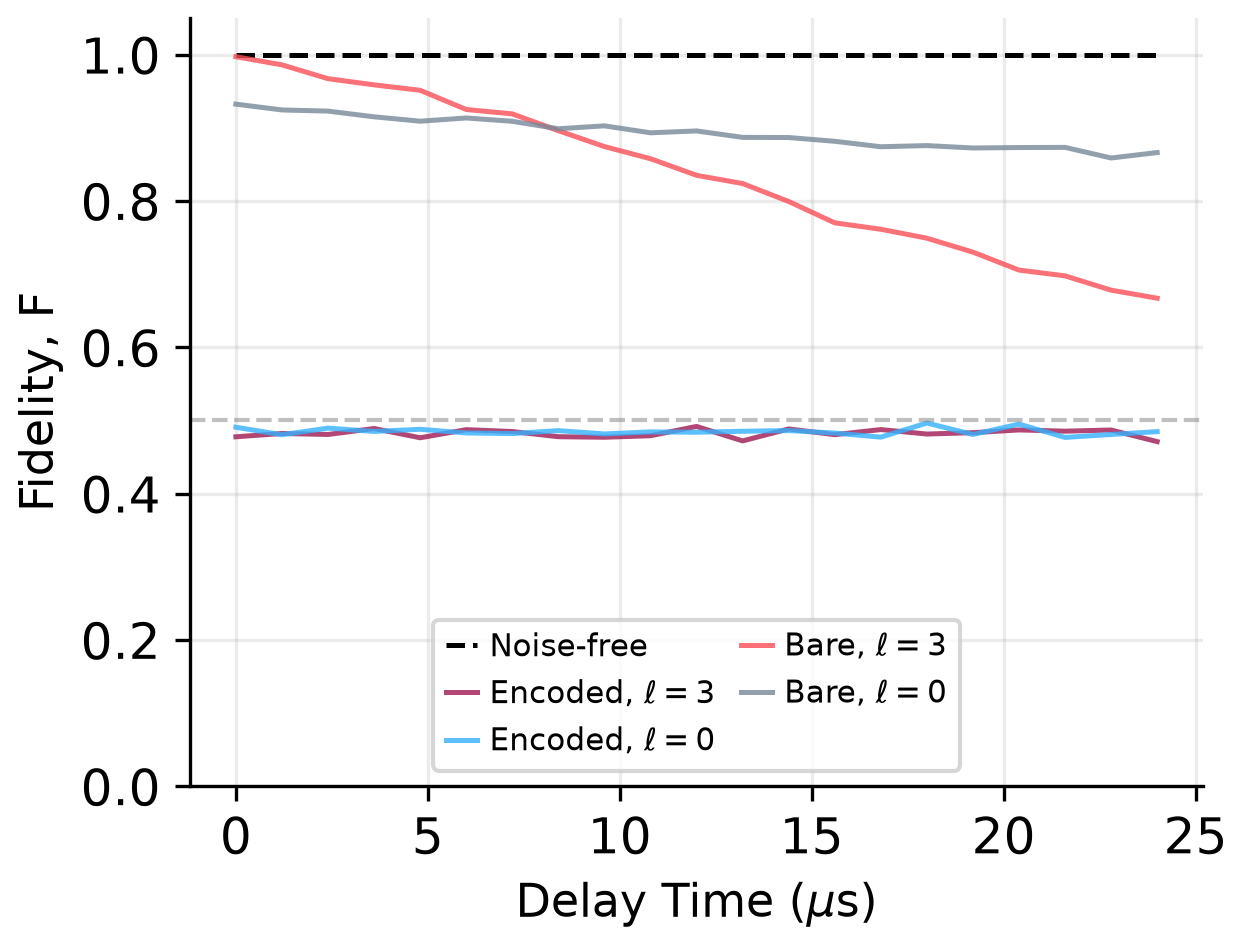
\includegraphics[width=\linewidth]{figure_02_qec_memory.png}
    \caption{Standalone single-qubit memory benchmark on IBM Kingston: encoded $[[5,1,3]]$ and bare runs at optimization levels 0 and 3. All four runs use $8192$ shots per point. They form an exploratory comparison between separate executions. The noise-free reference is the ideal-circuit result. These are not QEC-enhanced broadcasting data.}
    \label{QEC Fidelity}
\end{figure}

When QEC is enabled, each receiver qubit is replaced by a five-qubit $[[5,1,3]]$ block using the encoding tensor $E_{b_1 b_2 b_3 b_4 b_5, q}$, defined by $E[\ldots,0] = \ket{0_L}$ and $E[\ldots,1] = \ket{1_L}$.

\begin{figure*}[!tbp]
    \centering
    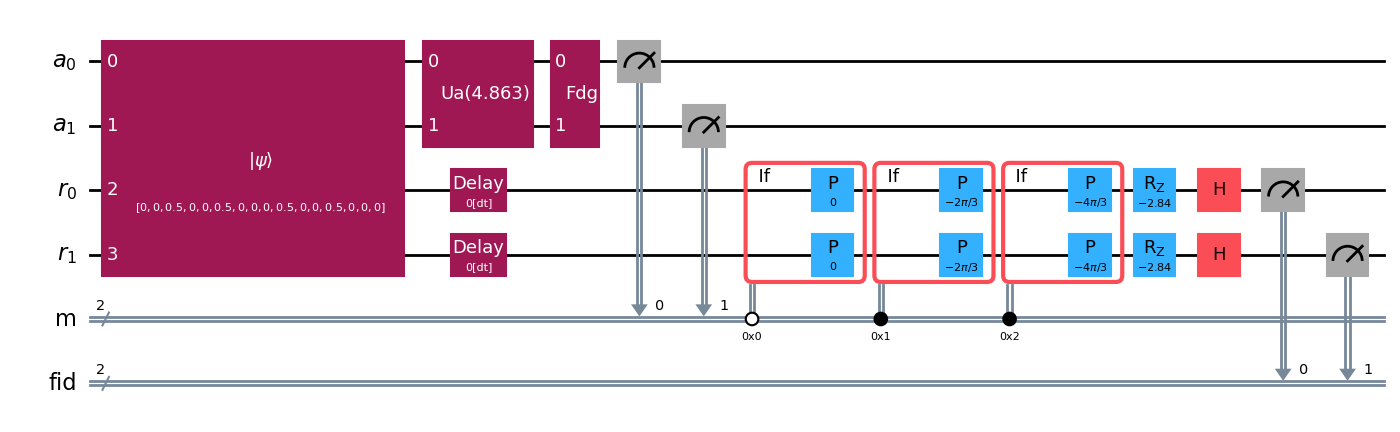
\includegraphics[width=0.95\linewidth]{m1n2qec0_circ.png}
    \caption{Exhaustive-feedforward circuit for $M{=}1$, $N{=}2$ without QEC. The sender qudit ($a_0, a_1$; two qubits encoding a qutrit) is initialized together with two receiver qubits ($r_0, r_1$) in the resource state $\ket{\Psi^{(1,2)}}$. After a parametric delay $\tau$, the sender phase gate $U_a(\theta)$ and inverse-DFT rotation $F_d^\dagger$ are applied, followed by a computational-basis measurement. Three conditional blocks (one per measurement outcome $n\in\{0,1,2\}$) each apply the corresponding phase correction $P(-2\pi n/3)$ to both receivers. Finally, $R_z(-\phi)$ and Hadamard gates rotate each receiver into the equatorial fidelity-measurement basis. An equivalent bitwise implementation uses two conditional blocks for valid sender outcomes, as described in the text.}
    \label{fig:circuit}
\end{figure*}

A schematic of the exhaustive-feedforward Qiskit circuit for the $M{=}1$, $N{=}2$ protocol without QEC is shown in Fig.~\ref{fig:circuit}. The circuit is built in six stages:

\begin{enumerate}
\item \textbf{State preparation.} The resource state $\ket{\Psi^{(M,N)}}$ (or its QEC-encoded variant) is loaded onto the sender register $\mathbf{a}$ ($M\cdot n_q$ qubits) and receiver register $\mathbf{r}$ ($N$ or $5N$ qubits).

\item \textbf{Delay.} A parametric delay $\tau$ is inserted on every receiver qubit. By sweeping $\tau$ we probe the effect of idle decoherence on the hardware.

\item \textbf{QEC recovery} (if enabled). Syndrome extraction and decoding are applied to each $[[5,1,3]]$ block reducing $5N$ physical qubits to $N$ decoded logical qubits.

\item \textbf{Sender phase gates.} Each sender~$j$ receives the diagonal unitary
\begin{align}
U_{a_j}(\theta_j) = \mathrm{diag}\!\left(e^{i(2k-N)\theta_j}\right)_{k=0}^{N},
\end{align}
on the first $N+1$ levels, extended by the identity on the unused levels of the $2^{n_q}$-dimensional register.

\item \textbf{Fourier measurement.} Each sender's $n_q$-qubit register is rotated by $F_d^\dagger$, the inverse DFT on $d = N{+}1$ levels, embedded in a $2^{n_q}$-dimensional unitary:
\begin{align}
F_d[n,k] = \frac{\omega^{nk}}{\sqrt{d}},\qquad \omega = e^{2\pi i/d},
\end{align}
followed by a computational-basis measurement. This is equivalent to measuring in the Fourier basis $\{\ket{u_n}\}$.

\item \textbf{Classical feedforward.} Write each measured value as $n_j=\sum_{b=0}^{n_q-1}2^b m_{jb}$. The bitwise implementation uses $Mn_q$ single-bit conditional blocks. When $m_{jb}=1$, each receiver receives $P(-2\pi2^b/(N+1))$, where $P(\lambda)=\operatorname{diag}(1,e^{i\lambda})$. These commuting rotations sum to the required correction, up to an overall phase.

\end{enumerate}

For valid sender values $0\le n_j\le N$, bitwise and exhaustive feedforward are equivalent. Hardware errors may populate unused binary values $n_j>N$. Bitwise feedforward applies the same linear phase formula to those values, whereas the exhaustive circuit skips correction if any value is invalid. Reported fidelities include all shots; invalid sender outcomes are not postselected. This difference in handling invalid values must be retained when comparing the two circuit implementations. Sender outcomes are recorded in register \texttt{m}; fidelity outcomes are recorded separately in \texttt{fid}. Separate histograms do not preserve sender--receiver shot correspondence, so conditional diagnostics require aligned records.

The $[[5,1,3]]$ error correction is implemented in the circuit using four shared ancilla qubits and Qiskit's dynamic-circuit primitives. In the gate-construction description below, Pauli-label characters are paired with qubits in their block-list order. Converting such a label into a Qiskit tensor-product matrix reverses the character order. Reversal preserves this code's stabilizer group, but the syndrome order must still follow the measured generators. For each five-qubit block the circuit appends three stages, described below.

Each stabilizer generator in Eq.~\eqref{eq:stabilizers} is measured using one ancilla qubit. For each Pauli factor $P_i$ in the generator acting on block qubit~$i$:
\begin{itemize}
\item If $P_i = X$: apply $H$ to qubit~$i$, then $\mathrm{CX}(i,\mathrm{anc})$, then $H$ again.
\item If $P_i = Y$: apply $S^\dagger$ and $H$ to qubit~$i$, then $\mathrm{CX}(i,\mathrm{anc})$, then $H$ and $S$.
\item If $P_i = Z$: apply $\mathrm{CX}(i,\mathrm{anc})$ directly.
\item If $P_i = I$: no gate.
\end{itemize}
The ancilla is then measured, yielding syndrome bit $s_r$. Ancilla qubits are reset before each stabilizer measurement and reused across blocks.

The four syndrome bits $s = (s_1, s_2, s_3, s_4)$ form a 4-bit integer where a precomputed lookup table maps each of the 16 possible syndrome values to the corresponding single-qubit Pauli correction (or identity for $s=0$). The appropriate Pauli gate ($X$, $Y$, or $Z$) is conditionally applied to the identified qubit. All 15 single-qubit Pauli errors on the five physical qubits produce distinct nonzero syndromes, guaranteeing correction of any weight-1 error~\cite{laflamme1996perfect,gottesman1997stabilizer}.

The decoding unitary $V_{\Enc}^\dagger$ is constructed as a $32\times 32$ matrix via Gram--Schmidt orthogonalization \cite{nielsen2010quantum}. The first two columns of the encoding matrix $W$ are the normalized logical basis vectors $\ket{0_L}$ and $\ket{1_L}$; the remaining 30 columns are filled from the standard basis to complete an orthonormal set. Then $V_{\Enc}^\dagger = W^\dagger$ maps
\begin{align}
V_{\Enc}^\dagger \ket{0_L} &= \ket{00000}, &
V_{\Enc}^\dagger \ket{1_L} &= \ket{00001},
\end{align}
so the decoded logical qubit resides on the first physical qubit in the Qiskit block list. Ket strings above place that qubit at the rightmost, least-significant position. In contrast, stabilizer labels in the extraction loop are read from left to right against the block list; the syndrome integer is $s_1+2s_2+4s_3+8s_4$. The lookup and extraction use this same ordering. Basis-vector reversal symmetry alone is insufficient to test ordering, so recovery and multi-receiver tests also exercise nontrivial states.

The generic state initialization and dense decoding unitary are retained implementation choices, with potentially large compilation overhead. Recovery and decoding precede sender operations in the library circuit; in the ideal protocol they can be moved past sender operations because they act on disjoint registers. Moving them in a hardware schedule can change idle and measurement exposure and is not assumed to preserve hardware fidelity.

The target output state for each receiver in the broadcasting protocol with $\alpha=\beta=1/\sqrt{2}$ lies on the equator of the Bloch sphere (the $XY$ plane):
\begin{align}
\ket{\psi_{\mathrm{target}}} = \frac{1}{\sqrt{2}}\!\left(e^{i\Phi}\ket{0} + e^{-i\Phi}\ket{1}\right),
\end{align}
where $\Phi = \sum_{j=1}^{M}\theta_j$ is the total sender angle.

We estimate the fidelity $F = \bra{\psi_{\mathrm{target}}}\rho_{\mathrm{out}}\ket{\psi_{\mathrm{target}}}$ using a single measurement basis per receiver qubit. Up to overall phases, the procedure appends two gates to each receiver qubit:
\begin{enumerate}
\item An $R_z(-\phi)$ rotation with $\phi = -2\Phi \bmod 2\pi$, which aligns the target state with $\ket{+}$:
\begin{align}
R_z(-\phi)\ket{\psi_{\mathrm{target}}} = \frac{1}{\sqrt{2}}\!\left(\ket{0} + \ket{1}\right) = \ket{+}.
\end{align}
\item A Hadamard gate $H$, which maps $\ket{+}\to\ket{0}$:
\begin{align}
H\,R_z(-\phi)\ket{\psi_{\mathrm{target}}} = \ket{0}.
\end{align}
\end{enumerate}
A computational-basis measurement is then performed. The probability of obtaining outcome~$0$ equals the fidelity:
\begin{align}
P(\text{outcome}=0) &= \bra{0}H\,R_z(-\phi)\,\rho_{\mathrm{out}}\,R_z(-\phi)^\dagger H^\dagger\ket{0} \nonumber \\
&= \bra{\psi_{\mathrm{target}}}\rho_{\mathrm{out}}\ket{\psi_{\mathrm{target}}} = F.
\end{align}
For a general real amplitude $\alpha$, the implementation instead applies $R_z(2\Phi)$ followed by $R_y[-2\arccos(\alpha)]$, mapping the target to $\ket{0}$. The supported numerical and hardware fidelity interface requires real $\alpha$, although the analytical factorization holds for complex normalized amplitudes. A single local measurement basis also retains the all-zero frequency and receiver-success covariance through the joint \texttt{fid} bitstrings; no additional measurement basis is needed for these quantities.

\begin{figure}[!tbp]
    \centering
    
\includegraphics[width=\linewidth]{figure_04_qec_crossover.png}
    \caption{Average receiver fidelity as a function of depolarizing probability $p$ for the $M{=}1$, $N{=}2$ protocol with and without $[[5,1,3]]$ quantum error correction compared against Monte Carlo trajectory sampling estimates. The inset resolves the low-noise crossing at $p_\star=(3-\sqrt6)/4$. The curves use $\alpha=1/\sqrt3$, $\theta=\pi/4$; local depolarizing fidelity is independent of this pure-target choice. The sampling curve is one fixed-sample run.}
    \label{qec_crossover}
\end{figure}

\begin{figure*}[!tbp]
    \centering
    
\includegraphics[width=\linewidth]{figure_05_delay_repeats.png}
    \caption{Receiver fidelity versus inserted delay for five separate unencoded $M=1,N=2$ runs at optimization level 3, grouped into two panels by backend. (a) Marrakesh: one sweep with $4096$ shots per point overlaid with three sweeps of $10{,}000$ shots per point at 121 delays spanning $0$--$24\,\mu\mathrm{s}$. (b) Kingston: one sweep with $10{,}000$ shots per point. Burgundy and cyan identify receiver 1 and receiver 2, and black dashed lines denote their mean within each run. Receiver curves and their means remain separate between runs. Delays use $dt=4$ ns, recorded for the Marrakesh runs and inferred from a separate Kingston memory measurement for the Kingston run.}
    \label{qiskit_delay}
\end{figure*}

\begin{figure*}[!tbp]
    \centering
    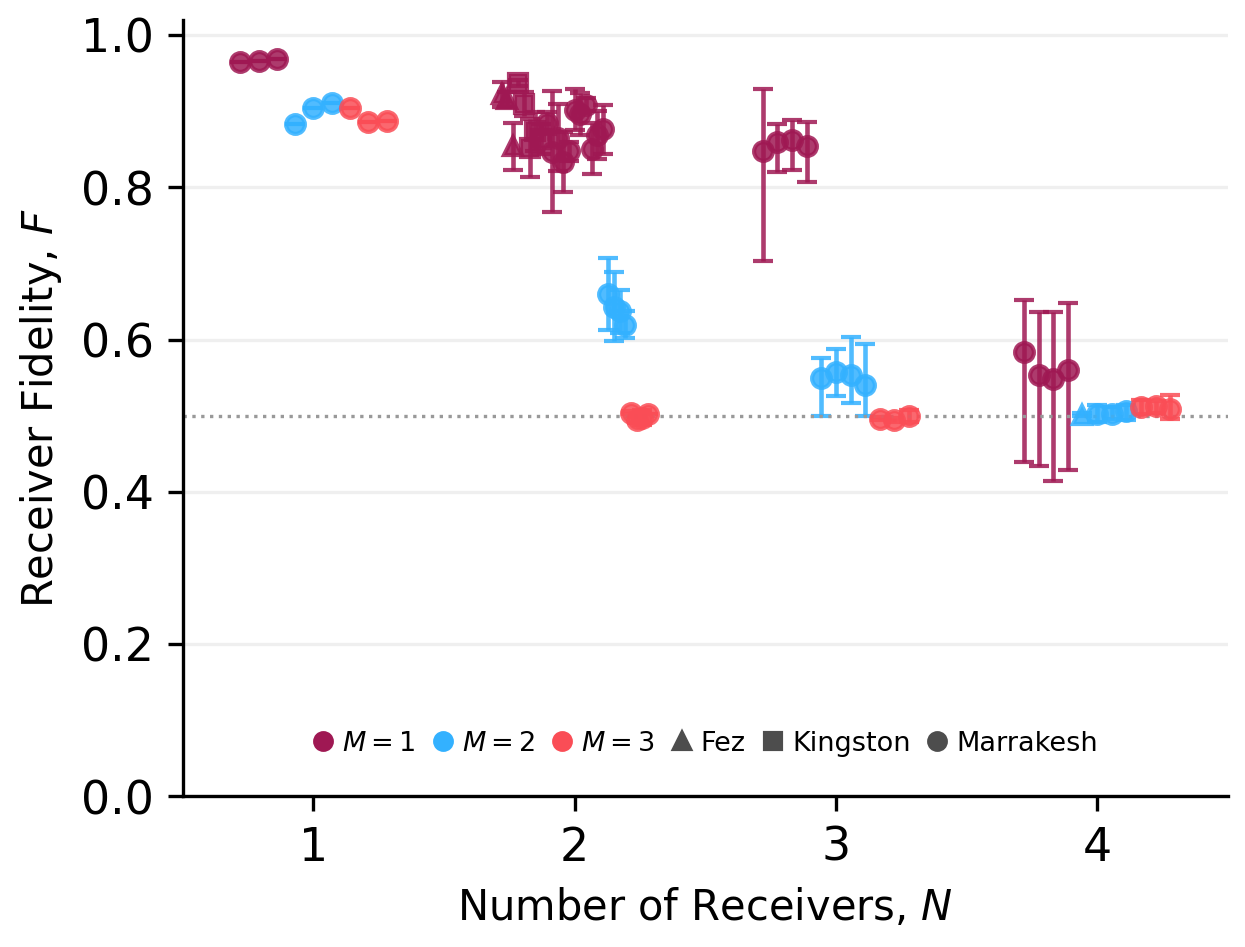
\includegraphics[width=\linewidth]{figure_06_hardware_scaling.png}
    \caption{Unencoded hardware observations at zero added delay and optimization level 3. The 55 points comprise 36 observations spanning $M=1,2,3$ and $N=1,2,3,4$ in three repetitions on IBM Marrakesh ($8192$ shots per case), three zero-delay observations from the Marrakesh delay sweeps ($10{,}000$ shots per point), and 16 further job/angle observations. Colour identifies sender count $M$ and marker shape identifies the backend. Each point is the receiver mean for one job, case and sender-angle tuple; its vertical bar spans the minimum and maximum receiver marginals. Bars describe receiver heterogeneity, not statistical uncertainty. Small horizontal offsets separate observations at the same integer $N$. The measurements span backends, shot counts, and circuit variants and are not pooled into a controlled scaling curve.}
    \label{protocol_scale}
\end{figure*}

\subsection{Analysis of hardware readouts}
The hardware data comprise 22 distinct broadcasting jobs containing 1218 per-angle, per-delay joint fidelity-register histograms, and five distinct standalone memory jobs. Duplicate observations are counted once, while separate cases within a job remain distinct. Counts are analyzed separately for each job, case, angle tuple, and delay.

Let $X_\ell$ be one when receiver $\ell$ reports zero in its target basis and zero otherwise. We estimate local fidelity by $\langle X_\ell\rangle$, joint fidelity by $\langle\prod_\ell X_\ell\rangle$, and worst-receiver fidelity by $\min_\ell\langle X_\ell\rangle$. Pair covariance is $C_{ij}=\langle X_iX_j\rangle-\langle X_i\rangle\langle X_j\rangle$, and receiver asymmetry is the paired difference $\Delta_{ij}=\langle X_i-X_j\rangle$. For $N=2$, $C_{12}$ equals joint fidelity minus the product of local fidelities. These operational success estimates include the imperfections of the measurement circuit and readout.

Local and joint confidence intervals use 95\% Wilson scores. Worst-receiver bounds use simultaneous Bonferroni-adjusted local intervals. Covariance, paired differences, and mean fidelity use multinomial delta-method intervals that retain within-shot receiver dependence. These intervals assume independent shots with fixed probabilities within one histogram. They exclude temporal correlation, calibration drift, readout bias, and between-job variation; the available measurements do not support tests of all of these assumptions. Intervals are not adjusted for searching across delays or receiver pairs.

For uniformly spaced delay traces with at least eight points, we compute a linearly detrended Hann-window periodogram separately for each receiver and the receiver mean at each angle tuple. We record its largest nonzero-frequency peak, frequency-bin spacing, and the variance explained by a sinusoid at that selected frequency after removing a linear trend. Peaks are descriptive: selection on the observed data is not a significance test, and ordered delay acquisition can confound delay with elapsed execution time.

\section{Results}

Figure~\ref{qec_crossover} compares exact bare and encoded simulations with a Pauli-trajectory estimate. The exact curves agree with their analytically predicted fidelities. The sampling curve provides a fixed-sample numerical comparison; the independently constructed stabilizer oracle and analytical factorization provide checks that do not rely on agreement between the two simulation paths alone. The low-noise QEC advantage ends at $p_\star\simeq0.1376$, as derived above.

Figure~\ref{qiskit_delay} overlays four unencoded $M=1,N=2$ Marrakesh delay sweeps in the left panel, with one Kingston sweep in the right panel. The three $10{,}000$-shot Marrakesh sweeps vary the sender phase and are retained separately. Their receiver-mean fidelities at zero added delay are $0.9023$, $0.8965$, and $0.9087$. The fidelity is already below one near zero added delay, so errors outside the inserted idle interval contribute materially. Differences between traces can reflect phase and execution differences as well as shot uncertainty. The Kingston receiver traces differ and exhibit nonmonotonic delay structure. A device-specific coherence-time explanation would require the calibration and layout associated with that execution; the available calibration data do not support assigning a particular $T_1$ range to this run.

At zero added delay in the Kingston run, the two receiver fidelities are $0.8941$ and $0.9257$. The worst-receiver interval is $[0.8870,0.9008]$; the joint fidelity is $0.8493$ with interval $[0.8422,0.8562]$. The success covariance is $0.02163$ with delta-method interval $[0.01882,0.02444]$, and the paired difference $F_1-F_2=-0.03160$ has interval $[-0.03840,-0.02480]$. Thus the recorded receiver imbalance is larger than the conditional shot uncertainty at this point, while its reproducibility across executions remains undetermined.

For the $4096$-shot Marrakesh sweep, the receiver mean at zero added delay is $0.8474$, worst-receiver fidelity is $0.8350$ with interval $[0.8216,0.8475]$, and joint fidelity is $0.7473$ with interval $[0.7338,0.7604]$. Its success covariance is $0.02936$ with interval $[0.02407,0.03466]$. This run remains a separate observation to retain backend and circuit differences. Positive measured covariance can arise from shared preparation, feedforward, readout, or drift as well as physical noise correlations, and cannot distinguish those mechanisms by itself.

The Kingston optimization-level-3 receiver-mean trace has a selected period of $0.504\,\mu\mathrm{s}$ with frequency-bin spacing $0.0413\,\mu\mathrm{s}^{-1}$. A sinusoid at this peak explains only $6.6\%$ of the linearly detrended variance. A separate level-0 trace gives $0.440\,\mu\mathrm{s}$ and $4.9\%$. Both peaks have only about two to three samples per cycle and lie near the Nyquist limit. Time conversion for these Kingston traces uses $dt$ inferred from a separate memory measurement on the same backend. The $4096$-shot Marrakesh trace instead uses its recorded $dt$; its dominant period is $24.2\,\mu\mathrm{s}$ over a $24\,\mu\mathrm{s}$ observation window, so it is unresolved against smooth drift. These spectral summaries do not establish a reproducible oscillation period or a dynamical-decoupling mechanism.

Figure~\ref{protocol_scale} shows 55 zero-delay observations spanning different sender and receiver counts. Of these, 36 cover all combinations of $M=1,2,3$ and $N=1,2,3,4$ in each of three jobs on IBM Marrakesh, with $8192$ shots per case and a separately retained sender-angle tuple per repetition. Three points come from the $10{,}000$-shot Marrakesh delay sweeps, and 16 are further job/angle observations. Measurements at the same $(M,N)$ remain separate. The combined display spans backends, shot counts, and circuit variants, so its points do not constitute a controlled scaling curve. Even within a matched group, a decrease in local fidelity with larger circuits can arise from accumulating independent gate, routing, idle, and readout errors. The prediction of $N$-independent local fidelity applies only to one idealized receiver channel per qubit, not to the full hardware circuit. These observations therefore do not establish correlated physical noise.

The library implements a complete QEC-enhanced broadcasting circuit, validated in simulation. The reported hardware QEC data in Fig.~\ref{QEC Fidelity} are the standalone encoded-memory benchmark; the measurements do not include a complete QEC-enhanced broadcasting hardware experiment.

\section{Conclusion}
Independent phase-covariant receiver channels produce the same product output in every sender branch of the restricted protocol for arbitrary $M,N$. The local and joint depolarizing fidelities then follow directly, including the exact $[[5,1,3]]$ logical-error polynomial and low-noise break-even probability. The classical sender outcomes are uniformly distributed independently of all phases; only the receivers' quantum states encode their sum. This statement concerns the ideal protocol and receiver-only noise, not cryptographic security against arbitrary devices or adversaries.

The hardware measurements show circuit overhead, receiver asymmetry, and delay-dependent structure. The standalone encoded-memory benchmark does not demonstrate an encoded fidelity advantage for its sampled settings, and the heterogeneous broadcasting observations cannot isolate a noise mechanism or establish a controlled scaling law. Analysis of the joint readouts yields joint fidelity, worst-receiver performance, success covariance, paired asymmetry, and descriptive delay spectra. These statistics establish features of the measured readouts; attribution to a physical noise mechanism requires matched circuit models and controlled repeats with preserved calibration, compiled circuits, and aligned shot records.

\section{Acknowledgements}
This research was supported by the National Science Foundation under the grant Collaborative Research: NeTS: Medium 2504622. Additionally it was supported in part, by a grant of computer time from the City University of New York High Performance Computing Center under NSF Grants CNS-0855217, CNS-0958379 and ACI-1126113. Additionally we are grateful for the feedback and advice of IBM's Dr. Olivia Lanes and Dr. Nick Bronn regarding our hardware fidelity results.

\bibliography{apssamp}

\end{document}
%
